% Options for packages loaded elsewhere
\PassOptionsToPackage{unicode}{hyperref}
\PassOptionsToPackage{hyphens}{url}
%
\documentclass[
]{article}
\usepackage{amsmath,amssymb}
\usepackage{iftex}
\ifPDFTeX
  \usepackage[T1]{fontenc}
  \usepackage[utf8]{inputenc}
  \usepackage{textcomp} % provide euro and other symbols
\else % if luatex or xetex
  \usepackage{unicode-math} % this also loads fontspec
  \defaultfontfeatures{Scale=MatchLowercase}
  \defaultfontfeatures[\rmfamily]{Ligatures=TeX,Scale=1}
\fi
\usepackage{lmodern}
\ifPDFTeX\else
  % xetex/luatex font selection
  \setmainfont[]{DejaVu Serif}
\fi
% Use upquote if available, for straight quotes in verbatim environments
\IfFileExists{upquote.sty}{\usepackage{upquote}}{}
\IfFileExists{microtype.sty}{% use microtype if available
  \usepackage[]{microtype}
  \UseMicrotypeSet[protrusion]{basicmath} % disable protrusion for tt fonts
}{}
\makeatletter
\@ifundefined{KOMAClassName}{% if non-KOMA class
  \IfFileExists{parskip.sty}{%
    \usepackage{parskip}
  }{% else
    \setlength{\parindent}{0pt}
    \setlength{\parskip}{6pt plus 2pt minus 1pt}}
}{% if KOMA class
  \KOMAoptions{parskip=half}}
\makeatother
\usepackage{xcolor}
\usepackage[margin=1in]{geometry}
\usepackage{graphicx}
\makeatletter
\def\maxwidth{\ifdim\Gin@nat@width>\linewidth\linewidth\else\Gin@nat@width\fi}
\def\maxheight{\ifdim\Gin@nat@height>\textheight\textheight\else\Gin@nat@height\fi}
\makeatother
% Scale images if necessary, so that they will not overflow the page
% margins by default, and it is still possible to overwrite the defaults
% using explicit options in \includegraphics[width, height, ...]{}
\setkeys{Gin}{width=\maxwidth,height=\maxheight,keepaspectratio}
% Set default figure placement to htbp
\makeatletter
\def\fps@figure{htbp}
\makeatother
\setlength{\emergencystretch}{3em} % prevent overfull lines
\providecommand{\tightlist}{%
  \setlength{\itemsep}{0pt}\setlength{\parskip}{0pt}}
\setcounter{secnumdepth}{-\maxdimen} % remove section numbering
\usepackage{booktabs}
\usepackage{caption}
\usepackage{longtable}
\usepackage{colortbl}
\usepackage{array}
\ifLuaTeX
  \usepackage{selnolig}  % disable illegal ligatures
\fi
\IfFileExists{bookmark.sty}{\usepackage{bookmark}}{\usepackage{hyperref}}
\IfFileExists{xurl.sty}{\usepackage{xurl}}{} % add URL line breaks if available
\urlstyle{same}
\hypersetup{
  pdftitle={Տնային տնտեսությունների վերլուծություն},
  pdfauthor={Աղասի Թավադյան},
  hidelinks,
  pdfcreator={LaTeX via pandoc}}

\title{Տնային տնտեսությունների վերլուծություն}
\author{Աղասի Թավադյան}
\date{2024-02-06}

\begin{document}
\maketitle

\href{https://www.tvyal.com/}{tvyal.com}\\
\href{https://www.tavadyan.com/}{tavadyan.com}

Այս վերլուծության բոլոր տվյալները վերցված են պաշտոնական աղբյուրներից,
մասնավորապես՝ \href{https://www.armstat.am/en/?nid=205}{տնային
տնտեսությունների կենսամակարդակի (կենսապայմանների) ամբողջացված
հետազոտության անվանազերծված միկրոտվյալների բազա (ըստ տնային
տնտեսությունների)},
\href{https://www.armstat.am/file/article/lab_market_2023_14.pdf}{Աշխատավարձի,
աշխատողների թվաքանակի և կազմակերպությունների թվի 2020-2022 ՀՀ
վիճակագրական կոմիտեի հաշվետվությունները} և
\href{https://www.cba.am/stat/stat_data_arm/6_CPI_arm.xls}{Հայաստանի
սպառողական գների ամսական ինդեքսը}: Տնային տնտեսությունների
կենսամակարդակի ցուցանիշները ինչպես նաև աշխատավարձերը ճշգրտվել են ամսական
կումուլատիվ գնաճով, այսինքն յուրաքանչյուր ցուցանիշ ներկայացնում է 2022
թվականի վերջի գնողունակությունը։ Տնային տնտեսությունների եկամուտների
ցուցանիշները նաև կշռվել են։ Հաշվարկները ամբողջությամբ հասանելի են
github-ում, դրանք կարելի է ստուգել այցելելով
\href{https://github.com/tavad/tvyal_newsletter/blob/main/2024/household_3_in_1.Rmd}{github-ի}
մեր էջը, որտեղ տրված են տվյալները, հաշվարկների և գծապատկերների կոդը։

\newpage

\section{Մաս 2. Ամուր ընտանիք՝ հարուստ
ընտանիք}\label{ux574ux561ux57d-2.-ux561ux574ux578ux582ux580-ux568ux576ux57fux561ux576ux56bux584-ux570ux561ux580ux578ux582ux57dux57f-ux568ux576ux57fux561ux576ux56bux584}

\subsection{Հայաստանի ընտանիքների ժողովրդագրական
վերլուծություն}\label{ux570ux561ux575ux561ux57dux57fux561ux576ux56b-ux568ux576ux57fux561ux576ux56bux584ux576ux565ux580ux56b-ux56aux578ux572ux578ux57eux580ux564ux561ux563ux580ux561ux56fux561ux576-ux57eux565ux580ux56cux578ux582ux56eux578ux582ux569ux575ux578ux582ux576}

\begin{quote}
Ոչ լիարժեք ընտանիք է համարվում մեկ ծնողից և երեխայից բաղկացած ընտանիքը:

Ոչ լիարժեք ընտանիքները բնութագրվում են հետևյալ հատկանիշներով՝

\begin{itemize}
\tightlist
\item
  որբացած,
\item
  ծնողազուրկ,
\item
  ամուսնալուծված։
\end{itemize}
\end{quote}

Դիտարկենք տնային տնտեսությունների եկամուտները ըստ դեցիլային խմբարի և այդ
խմբերում սեռատարիքային կազմի։

123 հազար դրամը չգերազանցող ամսական եկամուտ ունեցող ընտանիքները գտնվում
են 1-2 դեցիլային խմբերում։ Այս խմբին բնորոշ է տարեցների մեծ մասնաբաժինը,
որոնց ընտանիքների ավելի քան 35 տոկոսը բաղկացած է 63 և բարձր տարիքի
թոշակառուներից: Այս խմբի ընտանիքների միջին մեծությունը 2 մարդ է։ Այս
ընտանիքները հիմնականում լիարժեք չեն, այս խմբում միայն մեկ երրորդն է որ
ամուսին ունի: Երեխաների ամենացածր մասնաբաժինը նկատվում է այս խմբում,
աշխատունակ տարիքի անձանց ավելի ցածր կշռի հետ մեկտեղ:

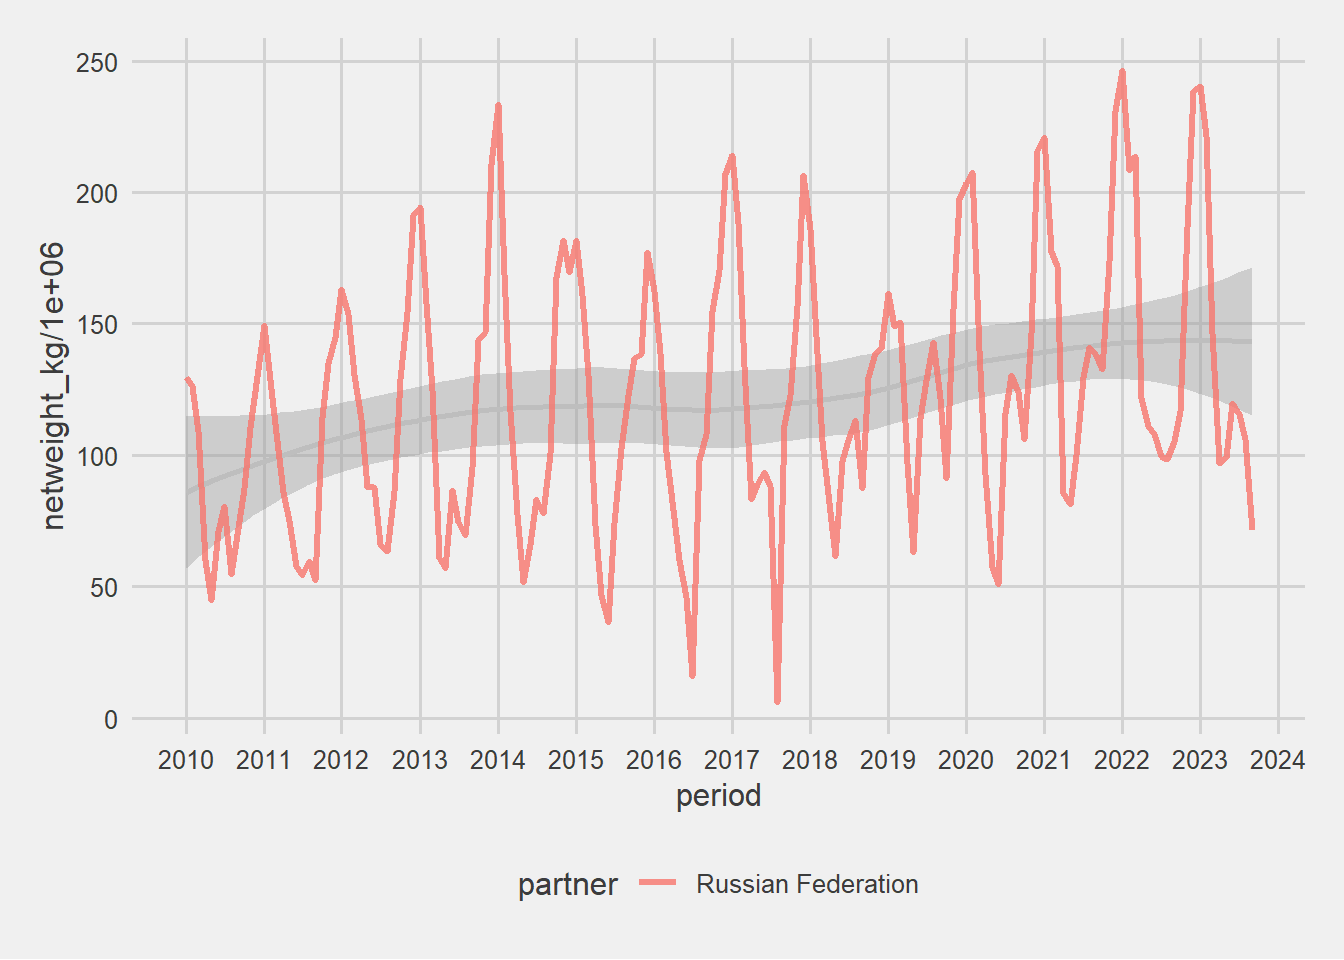
\includegraphics{household_3_in_1_files/figure-latex/unnamed-chunk-2-1.pdf}
\textbf{Գծապատկեր 2.1.} Տնային տնտեսությունների և տարիքային խմբարի
բաշխվածությունը

\begin{verbatim}
Դեցիլային խումբերը տվյալների բազան բաժանում են տասը հավասար մասերի,
որոնցից յուրաքանչյուրը ներկայացնում է ընդհանուր դիտարկումների 10%-ը՝
հավասար համամասնությամբ: Առաջին դեցիլը ներկայացնում է տվյալների 
առաջին 10%-ը, երկրորդը ներկայացնում է երկրորդ 10%-ը և այլն, 10-րդ դեցիլը, 
ներկայացնում է տվյալների ամենաբարձր 10%-ը:
\end{verbatim}

Ինչպես երևում է գծապատկերում ինչքան տնային տնտեսությունը ավելի քիչ է
ստանում եկամուտ, այնքան ավելի մեծ է հավանականությունը որ այդ տնային
տնտեսությունում տարեցների քանակությունը ավելի մեծ կլինի։ Այսպես 123
հազար դրամից ցածր եկամուտ ստացող տնային տնտեսություններում 1/3-ը 63 և
ավել տարիք ունեցող քաղաքացիներ են։ Այսպես այս խմբի վրա ավելի շատ են
ընկնում առողջապահական ծախսերը:

Որքան մեծ է տնային տնտեսության գլխի տարիքը և որքան մեծ է տնային
տնտեսության գլխի կին լինելու հավանականությունը, այնքան մեծ է ընտանիքի
անապահով խավի մեջ հայտնվելու հավանականությունը: Անապահով տնային
տնտեսությունները հիմնականում բաղկացած են տարեց կանանցից, ովքեր չունեն
հարազատներ, որոնց մոտ 40 տոկոսն ունի հիմնական կրթություն:

Հարուստ խավն առանձնանում է ավելի մեծ ընտանիքներով, ինչի մասին է վկայում
10-րդ դեցիլային խմբում միջինը 5 հոգանոց ընտանիքների չափը։ Ապահովված
տնային տնտեսություններն ունեն նաև աշխատողների մեծ թվով անդամներ, որոնցից
երեքից ավելի անդամներ գտնվում են աշխատանքային տարիքում: Ավելին՝ ապահով
ընտանիքների գլուխների ավելի քան 77 տոկոսն ունի ամուսին։ Այսպիսով,
ամբողջական ընտանիքի առկայությունը հիմնականում բնութագրում է ապահովված
ընտանիք: Կրթության մակարդակն ամենաբարձրն է 10-րդ դեցիլում, որի 56,3
տոկոսն ունի հիմնական կրթություն:

Միջին խավը հասարակության հիմքն է։ Այս խավն ունի ամենաշատ երեխաների թիվը։
Այս ընտանիքների անդամների մոտավորապես 25 տոկոսը երեխաներ են՝ ի
տարբերություն հարուստ խավի, որը համեմատաբար ավելի քիչ երեխաներ ունի։
Ամենաապահով 10-րդ դեցիլային խմբում երեխաների տոկոսը կազմում է 21 տոկոս։

Ամբողջական ընտանիքի առկայությունը էականորեն ազդում է ապահով և միջին խավի
ձևավորման վրա, մինչդեռ ցածր խավին առավելապես բնորոշ է միայնությունը։

\textbf{Աղյուսակ 2.1.} ՀՀ տնային տնտեսությունների ժողովրդագրական
վերլուծություն

\setlength{\LTpost}{0mm}
\begin{longtable}{crrrrrrrrrrr}
\caption*{
{\large Armenia's Household Demographics} \\ 
{\small Summary of demographic and income information in 2022}
} \\ 
\toprule
 &  & \multicolumn{3}{c}{Demographic Information} & \multicolumn{3}{c}{Household Composition (Average)} & \multicolumn{4}{c}{Head of Household (HH) Details} \\ 
\cmidrule(lr){3-5} \cmidrule(lr){6-8} \cmidrule(lr){9-12}
Household Decile & Average Monthly Income (in thousand AMD) & Working-Age Population (\%) & Senior Population (over 63, \%) & Child Population (0-17, \%) & Household Size & Working-Age & Children & Average Age of HH & Proportion of Female in HH (\%) & HH with Basic Education (\%) & Married HH (\%) \\ 
\midrule\addlinespace[2.5pt]
1 & \cellcolor[HTML]{F95D6A}{\textcolor[HTML]{FFFFFF}{$65.9$}} & \cellcolor[HTML]{FFC9C3}{\textcolor[HTML]{000000}{$52.9$%}} & \cellcolor[HTML]{FF9595}{\textcolor[HTML]{000000}{$33.6$%}} & \cellcolor[HTML]{F95D6A}{\textcolor[HTML]{FFFFFF}{$13.5$%}} & \cellcolor[HTML]{F95D6A}{\textcolor[HTML]{FFFFFF}{$1.86$}} & \cellcolor[HTML]{F95D6A}{\textcolor[HTML]{FFFFFF}{$0.98$}} & \cellcolor[HTML]{F95D6A}{\textcolor[HTML]{FFFFFF}{$0.25$}} & \cellcolor[HTML]{FD7178}{\textcolor[HTML]{FFFFFF}{$65$}} & \cellcolor[HTML]{F95D6A}{\textcolor[HTML]{FFFFFF}{$68.6$%}} & \cellcolor[HTML]{FB6771}{\textcolor[HTML]{FFFFFF}{$40.6$%}} & \cellcolor[HTML]{F95D6A}{\textcolor[HTML]{FFFFFF}{$23.8$%}} \\ 
2 & \cellcolor[HTML]{FD7379}{\textcolor[HTML]{FFFFFF}{$105.0$}} & \cellcolor[HTML]{F95D6A}{\textcolor[HTML]{FFFFFF}{$46.9$%}} & \cellcolor[HTML]{F95D6A}{\textcolor[HTML]{FFFFFF}{$37.5$%}} & \cellcolor[HTML]{FF9493}{\textcolor[HTML]{000000}{$15.6$%}} & \cellcolor[HTML]{FF8789}{\textcolor[HTML]{000000}{$2.24$}} & \cellcolor[HTML]{FB6871}{\textcolor[HTML]{FFFFFF}{$1.05$}} & \cellcolor[HTML]{FF8587}{\textcolor[HTML]{000000}{$0.35$}} & \cellcolor[HTML]{F95D6A}{\textcolor[HTML]{FFFFFF}{$66$}} & \cellcolor[HTML]{FFC2BD}{\textcolor[HTML]{000000}{$53.1$%}} & \cellcolor[HTML]{FA656F}{\textcolor[HTML]{FFFFFF}{$40.5$%}} & \cellcolor[HTML]{FFBFBA}{\textcolor[HTML]{000000}{$39.8$%}} \\ 
3 & \cellcolor[HTML]{FF8789}{\textcolor[HTML]{000000}{$143.1$}} & \cellcolor[HTML]{FFA09E}{\textcolor[HTML]{000000}{$50.5$%}} & \cellcolor[HTML]{FFB9B4}{\textcolor[HTML]{000000}{$31.0$%}} & \cellcolor[HTML]{FFD9D3}{\textcolor[HTML]{000000}{$18.5$%}} & \cellcolor[HTML]{FFB8B4}{\textcolor[HTML]{000000}{$2.72$}} & \cellcolor[HTML]{FF9897}{\textcolor[HTML]{000000}{$1.37$}} & \cellcolor[HTML]{FFBEB9}{\textcolor[HTML]{000000}{$0.50$}} & \cellcolor[HTML]{FFA3A1}{\textcolor[HTML]{000000}{$64$}} & \cellcolor[HTML]{FFFCF5}{\textcolor[HTML]{000000}{$43.4$%}} & \cellcolor[HTML]{F95D6A}{\textcolor[HTML]{FFFFFF}{$40.2$%}} & \cellcolor[HTML]{F1EFED}{\textcolor[HTML]{000000}{$52.4$%}} \\ 
4 & \cellcolor[HTML]{FF9C9A}{\textcolor[HTML]{000000}{$186.0$}} & \cellcolor[HTML]{FFEFE8}{\textcolor[HTML]{000000}{$55.2$%}} & \cellcolor[HTML]{D2D3DB}{\textcolor[HTML]{000000}{$23.2$%}} & \cellcolor[HTML]{CECFD8}{\textcolor[HTML]{000000}{$21.6$%}} & \cellcolor[HTML]{FFE3DC}{\textcolor[HTML]{000000}{$3.17$}} & \cellcolor[HTML]{FFCBC5}{\textcolor[HTML]{000000}{$1.75$}} & \cellcolor[HTML]{FEFBF4}{\textcolor[HTML]{000000}{$0.68$}} & \cellcolor[HTML]{F0EFEC}{\textcolor[HTML]{000000}{$62$}} & \cellcolor[HTML]{CBCCD6}{\textcolor[HTML]{000000}{$37.2$%}} & \cellcolor[HTML]{FF8D8E}{\textcolor[HTML]{000000}{$42.4$%}} & \cellcolor[HTML]{CBCCD6}{\textcolor[HTML]{000000}{$57.4$%}} \\ 
5 & \cellcolor[HTML]{FFB1AD}{\textcolor[HTML]{000000}{$231.3$}} & \cellcolor[HTML]{FFE2DB}{\textcolor[HTML]{000000}{$54.4$%}} & \cellcolor[HTML]{9FA5BC}{\textcolor[HTML]{000000}{$20.2$%}} & \cellcolor[HTML]{596A92}{\textcolor[HTML]{FFFFFF}{$25.4$%}} & \cellcolor[HTML]{E6E5E6}{\textcolor[HTML]{000000}{$3.62$}} & \cellcolor[HTML]{FFE8E1}{\textcolor[HTML]{000000}{$1.97$}} & \cellcolor[HTML]{8E96B2}{\textcolor[HTML]{FFFFFF}{$0.92$}} & \cellcolor[HTML]{B4B8C8}{\textcolor[HTML]{000000}{$61$}} & \cellcolor[HTML]{B9BCCB}{\textcolor[HTML]{000000}{$35.0$%}} & \cellcolor[HTML]{FF9C9B}{\textcolor[HTML]{000000}{$43.1$%}} & \cellcolor[HTML]{B4B8C8}{\textcolor[HTML]{000000}{$60.3$%}} \\ 
6 & \cellcolor[HTML]{FFC7C1}{\textcolor[HTML]{000000}{$277.4$}} & \cellcolor[HTML]{B8BBCA}{\textcolor[HTML]{000000}{$59.0$%}} & \cellcolor[HTML]{7C87A7}{\textcolor[HTML]{FFFFFF}{$18.2$%}} & \cellcolor[HTML]{AAAFC2}{\textcolor[HTML]{000000}{$22.8$%}} & \cellcolor[HTML]{D0D1D9}{\textcolor[HTML]{000000}{$3.78$}} & \cellcolor[HTML]{EAE8E8}{\textcolor[HTML]{000000}{$2.23$}} & \cellcolor[HTML]{A9AEC2}{\textcolor[HTML]{000000}{$0.86$}} & \cellcolor[HTML]{5A6A93}{\textcolor[HTML]{FFFFFF}{$59$}} & \cellcolor[HTML]{6F7C9F}{\textcolor[HTML]{FFFFFF}{$25.8$%}} & \cellcolor[HTML]{FFEFE8}{\textcolor[HTML]{000000}{$47.5$%}} & \cellcolor[HTML]{65739A}{\textcolor[HTML]{FFFFFF}{$70.8$%}} \\ 
7 & \cellcolor[HTML]{FFE2DB}{\textcolor[HTML]{000000}{$336.5$}} & \cellcolor[HTML]{CFD0D8}{\textcolor[HTML]{000000}{$58.0$%}} & \cellcolor[HTML]{4A5E8A}{\textcolor[HTML]{FFFFFF}{$15.3$%}} & \cellcolor[HTML]{2F4B7C}{\textcolor[HTML]{FFFFFF}{$26.7$%}} & \cellcolor[HTML]{9FA5BC}{\textcolor[HTML]{000000}{$4.16$}} & \cellcolor[HTML]{C8CAD4}{\textcolor[HTML]{000000}{$2.42$}} & \cellcolor[HTML]{314C7D}{\textcolor[HTML]{FFFFFF}{$1.11$}} & \cellcolor[HTML]{2F4B7C}{\textcolor[HTML]{FFFFFF}{$58$}} & \cellcolor[HTML]{7480A2}{\textcolor[HTML]{FFFFFF}{$26.5$%}} & \cellcolor[HTML]{FFD6D0}{\textcolor[HTML]{000000}{$46.2$%}} & \cellcolor[HTML]{7580A2}{\textcolor[HTML]{FFFFFF}{$68.8$%}} \\ 
8 & \cellcolor[HTML]{F5F3EF}{\textcolor[HTML]{000000}{$409.8$}} & \cellcolor[HTML]{A4AABF}{\textcolor[HTML]{000000}{$59.9$%}} & \cellcolor[HTML]{485C89}{\textcolor[HTML]{FFFFFF}{$15.2$%}} & \cellcolor[HTML]{68759B}{\textcolor[HTML]{FFFFFF}{$24.9$%}} & \cellcolor[HTML]{7783A4}{\textcolor[HTML]{FFFFFF}{$4.47$}} & \cellcolor[HTML]{99A0B8}{\textcolor[HTML]{FFFFFF}{$2.68$}} & \cellcolor[HTML]{2F4B7C}{\textcolor[HTML]{FFFFFF}{$1.11$}} & \cellcolor[HTML]{6C799D}{\textcolor[HTML]{FFFFFF}{$59$}} & \cellcolor[HTML]{6A789C}{\textcolor[HTML]{FFFFFF}{$25.2$%}} & \cellcolor[HTML]{FFF4ED}{\textcolor[HTML]{000000}{$47.8$%}} & \cellcolor[HTML]{627197}{\textcolor[HTML]{FFFFFF}{$71.3$%}} \\ 
9 & \cellcolor[HTML]{B1B5C6}{\textcolor[HTML]{000000}{$517.6$}} & \cellcolor[HTML]{8790AD}{\textcolor[HTML]{FFFFFF}{$61.2$%}} & \cellcolor[HTML]{54658F}{\textcolor[HTML]{FFFFFF}{$15.8$%}} & \cellcolor[HTML]{A5AABF}{\textcolor[HTML]{000000}{$23.0$%}} & \cellcolor[HTML]{4A5E8A}{\textcolor[HTML]{FFFFFF}{$4.81$}} & \cellcolor[HTML]{69769C}{\textcolor[HTML]{FFFFFF}{$2.95$}} & \cellcolor[HTML]{354F7F}{\textcolor[HTML]{FFFFFF}{$1.10$}} & \cellcolor[HTML]{808AA9}{\textcolor[HTML]{FFFFFF}{$60$}} & \cellcolor[HTML]{334E7E}{\textcolor[HTML]{FFFFFF}{$18.7$%}} & \cellcolor[HTML]{E7E6E6}{\textcolor[HTML]{000000}{$49.2$%}} & \cellcolor[HTML]{324D7D}{\textcolor[HTML]{FFFFFF}{$77.3$%}} \\ 
10 & \cellcolor[HTML]{2F4B7C}{\textcolor[HTML]{FFFFFF}{$722.6$}} & \cellcolor[HTML]{2F4B7C}{\textcolor[HTML]{FFFFFF}{$65.0$%}} & \cellcolor[HTML]{2F4B7C}{\textcolor[HTML]{FFFFFF}{$13.9$%}} & \cellcolor[HTML]{DDDDE1}{\textcolor[HTML]{000000}{$21.2$%}} & \cellcolor[HTML]{2F4B7C}{\textcolor[HTML]{FFFFFF}{$5.00$}} & \cellcolor[HTML]{2F4B7C}{\textcolor[HTML]{FFFFFF}{$3.25$}} & \cellcolor[HTML]{4C608B}{\textcolor[HTML]{FFFFFF}{$1.06$}} & \cellcolor[HTML]{606F96}{\textcolor[HTML]{FFFFFF}{$59$}} & \cellcolor[HTML]{2F4B7C}{\textcolor[HTML]{FFFFFF}{$18.3$%}} & \cellcolor[HTML]{2F4B7C}{\textcolor[HTML]{FFFFFF}{$56.3$%}} & \cellcolor[HTML]{2F4B7C}{\textcolor[HTML]{FFFFFF}{$77.5$%}} \\ 
\bottomrule
\end{longtable}
\begin{minipage}{\linewidth}
    |    Data Source: armstat.am\\
\end{minipage}

Ինչպես երևում է մինչև 161 հազար դրամ ընդհանուր եկամուտ ստացող առաջին,
երկրորդ և երրորդ դեցիլային խմբերի հիմնական դրամական եկամուտը գոյանում է
կնսաթոշակից։*

Տնային տնտեսությունների ամենաաղքատ 10 տոկոսի հիմնական եկամտի աղբյուրը
կենսաթոշակն է, որը կազմում է մինչև 85 հազար դրամ ստացող տնային
տնտեսությունների եկամտի 67 տոկոսը, 12 տոկոսը՝ ընտանեկան նպաստն է, իսկ
աշխատավարձը՝ ընդամենը 7 տոկոսը։ Նշենք որ այս խմբում մեկ տնային
տնտեսության հաշվով կենսաթոշակից միջին եկամուտը կազմում է 28 հազար դրամ։
Սա չի նշանակում որ այս խմբի թոշակառուները միջինը ստանում են 28 հազար
դրամ։ Պարզապես որոշ տնային տնտեսություններ այս խմբում չունեն 63 անց
թոշակառու և այդ տնային տնտեսությունները կենսաթոշակ չեն ստանում։ Նույնը
վերաբերում է աշխատավարձից ստացված միջին եկամտին։ Ըստ տնային
տնտեսությունների բազայի 2022-ին 63 անց թոշակառուների մոտ միջին
կենսաթոշակը կազմում է 46 245 դրամ։

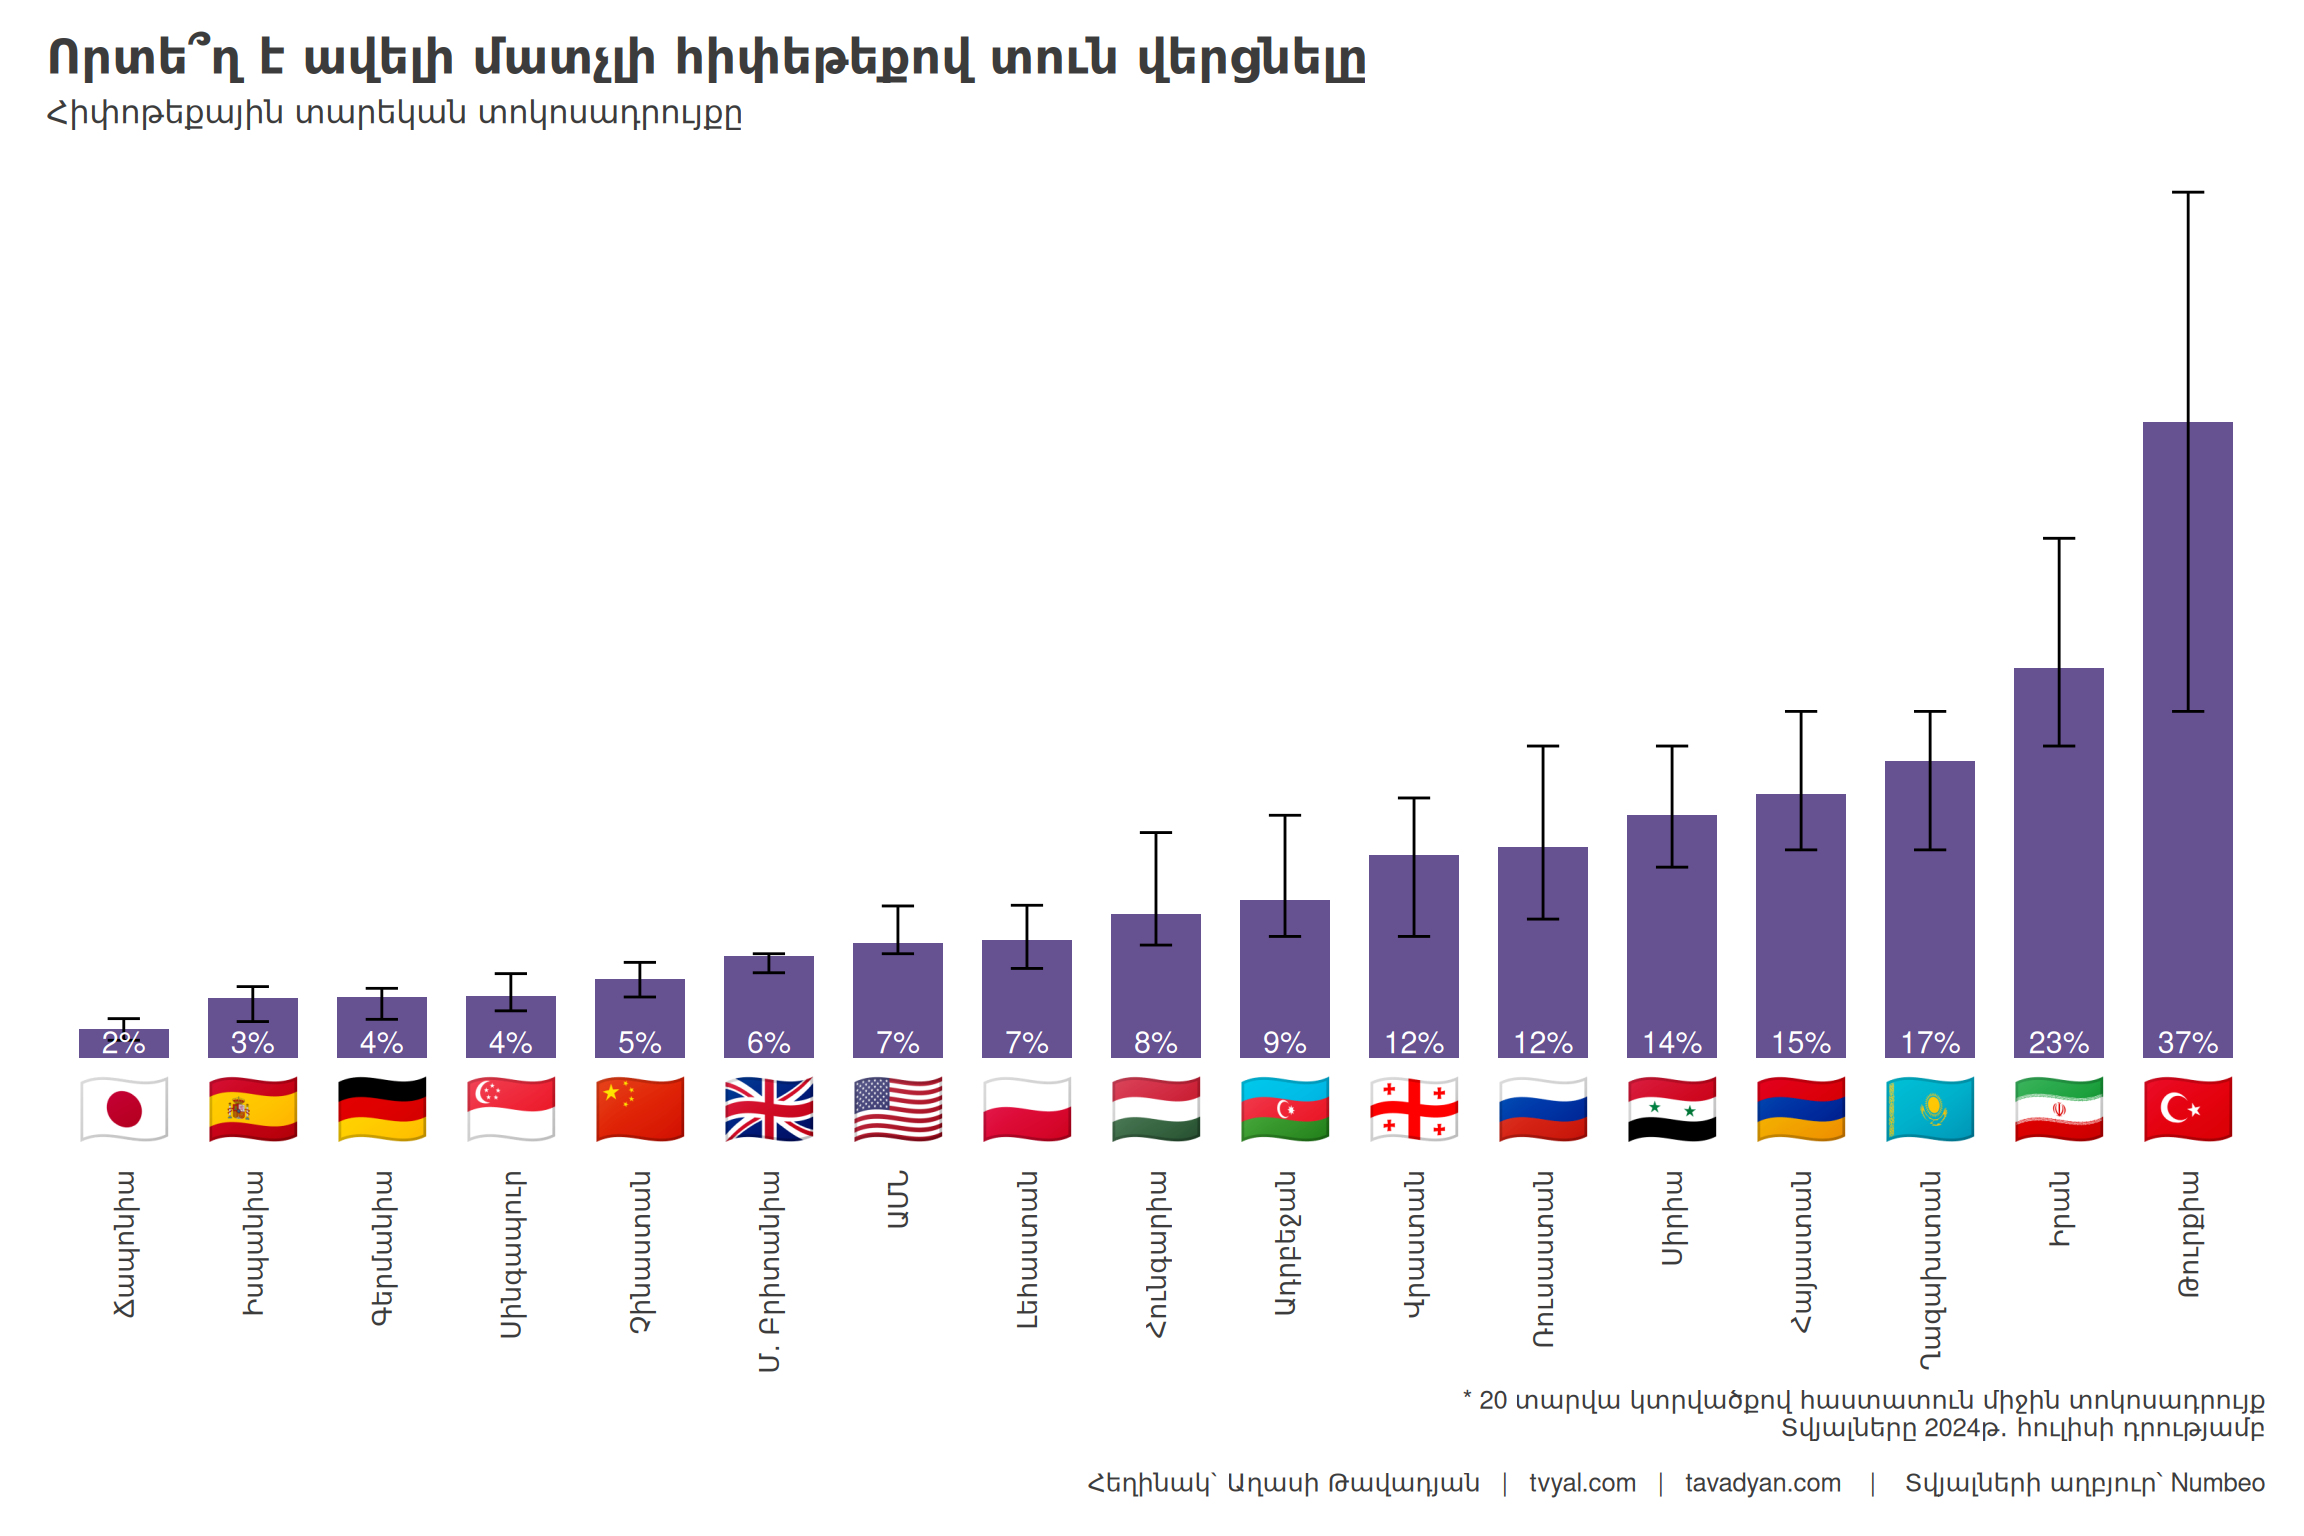
\includegraphics{household_3_in_1_files/figure-latex/unnamed-chunk-4-1.pdf}
\textbf{Գծապատկեր 2.2.} Դեցիլային խմբերի եկամտների աղբյուրները, դրամ

3-ից 5-րդ դեցիլային խմբերի դրամական եկամուտի ավելի քան 10 տոկոսը ստանում
են բարեկամներից, որոնք գտնվում են արտասահմանում։ Սա ամենամեծ տեսակարար
կշիռն է։ Այս եկամուտը ստացվում է արտագնա աշխատողներից։

Ինչքան տնային տնտեսությունը ապահով է այնքան մեծանում է
ինքնազբաղվածությունից կամ բիզնեսից ստացված եկամուտի մասնաբաժինը։
Հուշագրավ է այն որ 10-րդ խմբում, որը ներկայացնում է ամենաապահով 10
տոկոսը, աշխատավարձից ստացված եկամուտի տոկոսային կշիռը ավելի ցածր է, քան
9-րդ խմբում։ Ամենաապահով խավը առանձնանում է ինքնազբաղվածների համեմատաբար
մեծ տոկոսով։ Նշենք նաև որ այս խմբի եկամտների 1 տոկոսը ձևավորվում է
անշարժ գույքի վաճառքից, որը գծապատկերում ներառված է ``այլ եկամուտներ''
սանդղակում։

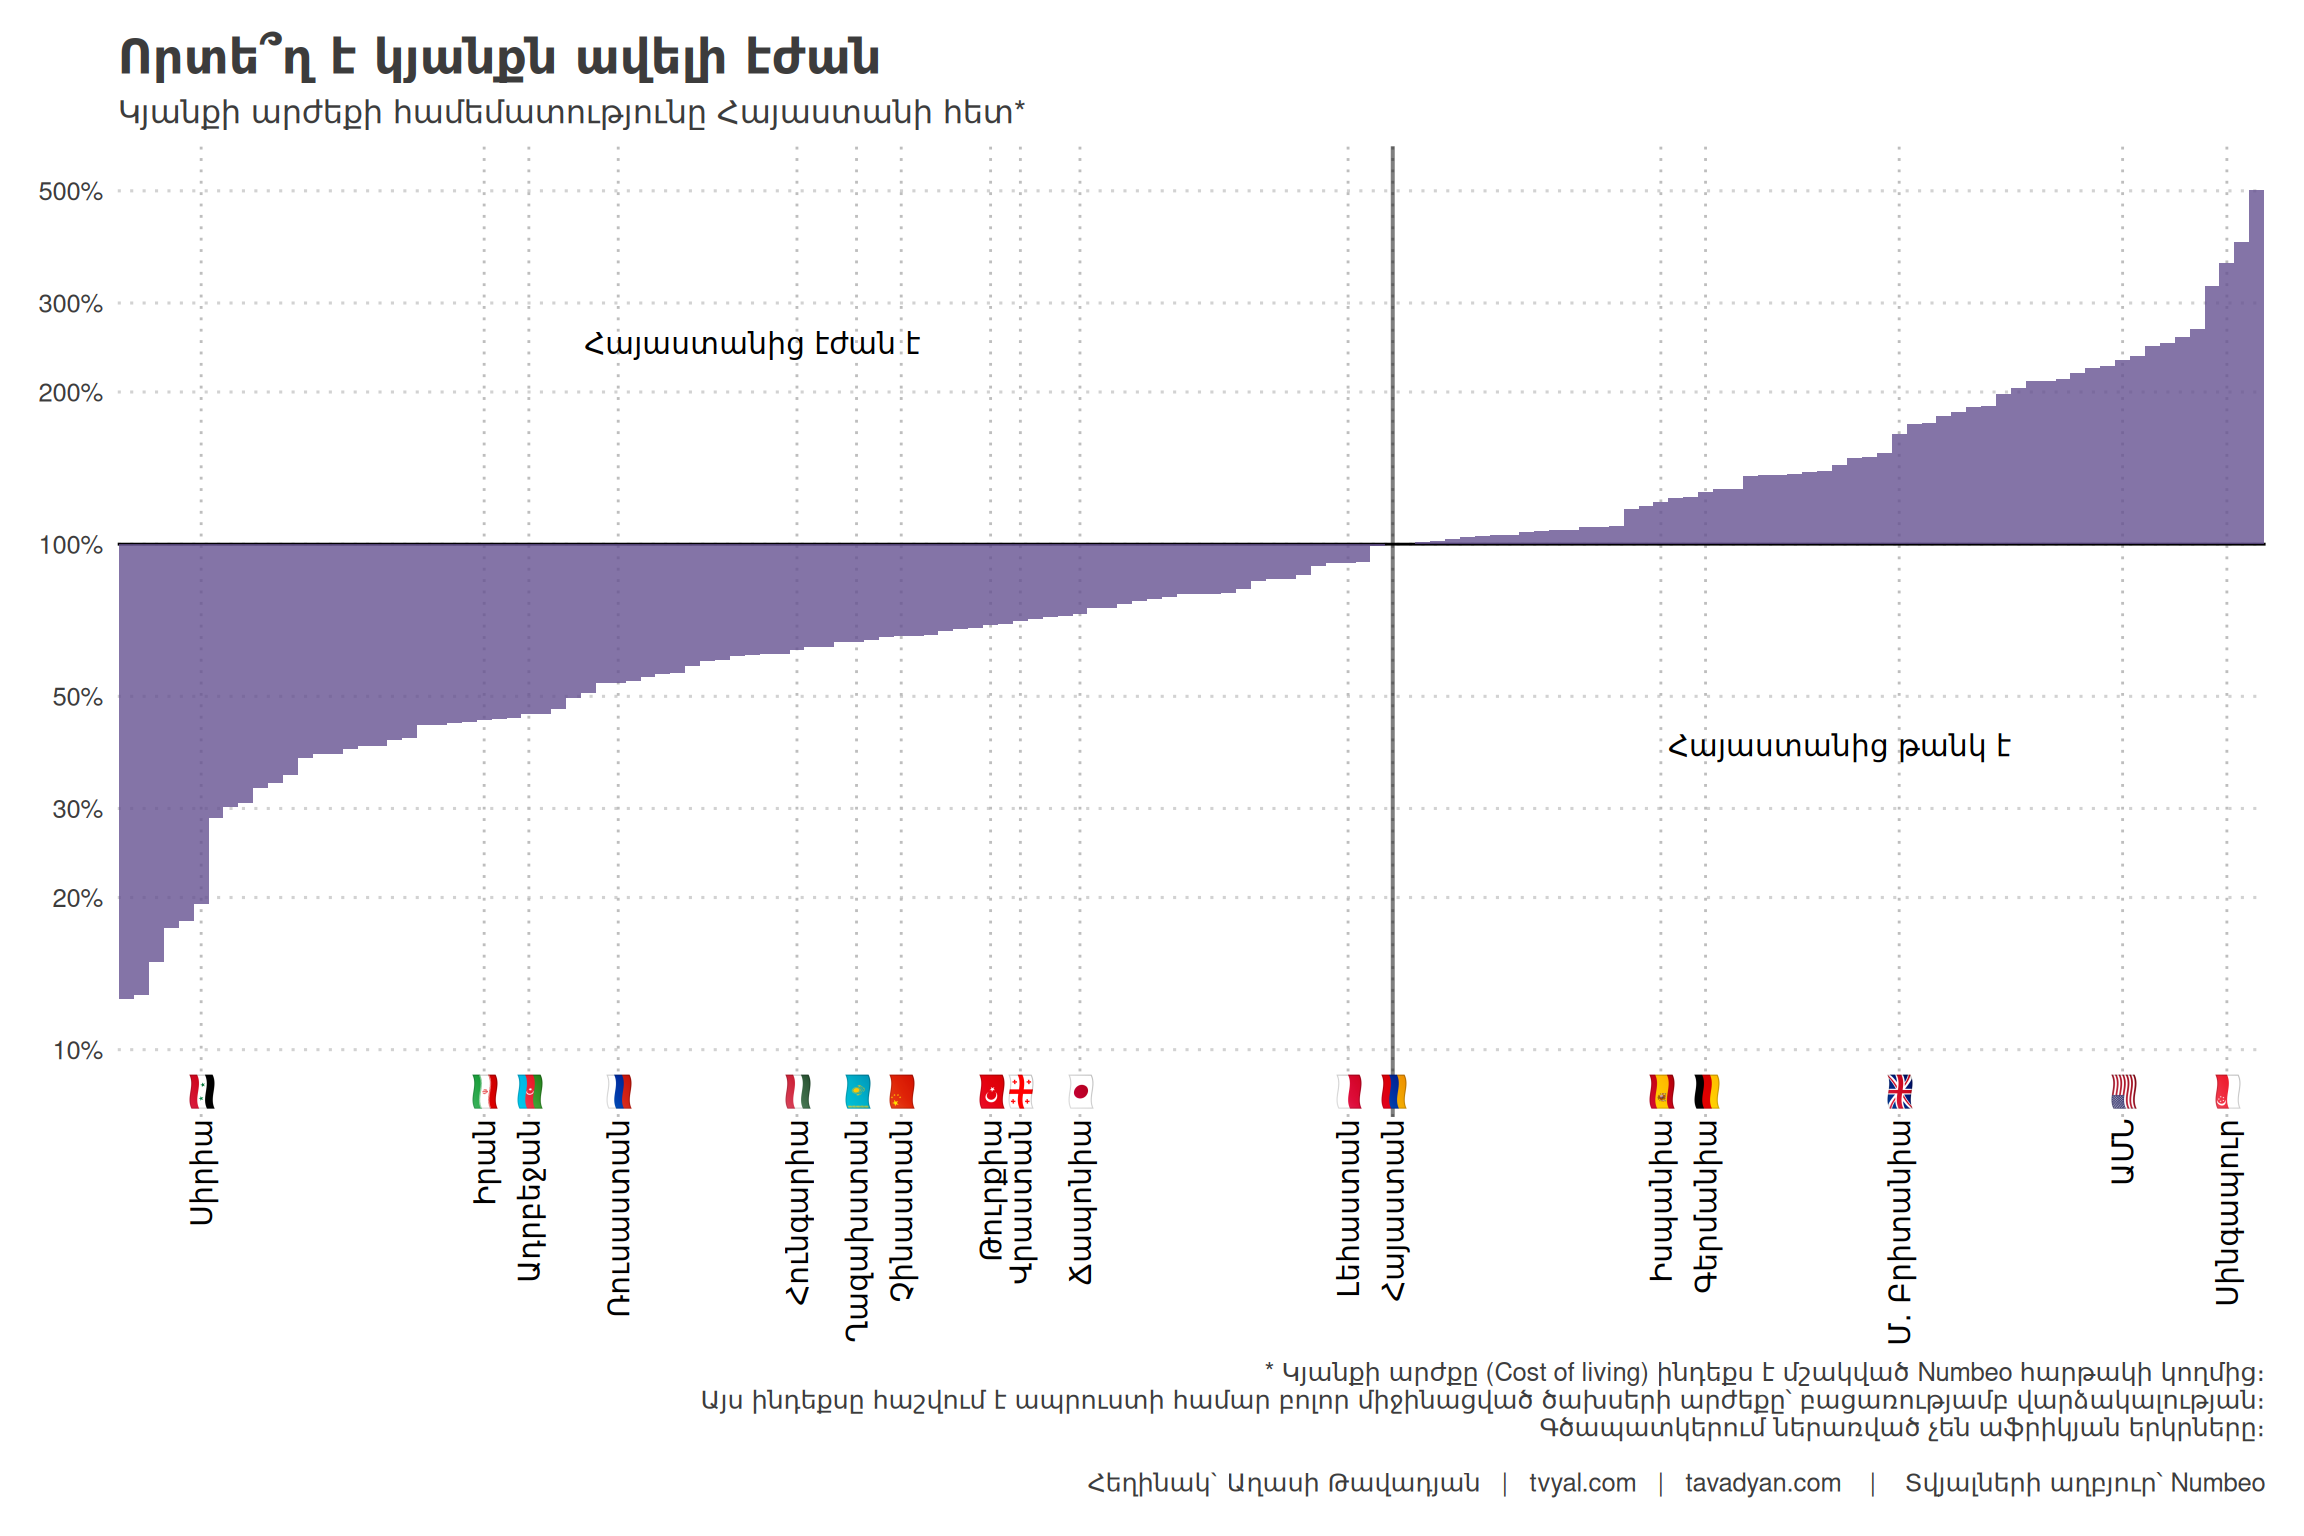
\includegraphics{household_3_in_1_files/figure-latex/unnamed-chunk-5-1.pdf}
\textbf{Գծապատկեր 2.3.} Դեցիլային խմբերի եկամտների աղբյուրները, տոկոս

*Նշում․ Տնային տնտեսությունների եկամուտները ձևավորվում են դրամական և ոչ
դրամական աղբյուրներից։ Դեցիլային խմբերը հաշվարկվել են ընդհանուր եկամտի
հիման վրա։ 2-րդ և 3-րդ գծապատկերները արտացոլում են միայն դրամական
եկամուտների բաշխվածությունը ըստ խմբերի։ Առաջին աղյուսակի դեցիլային
խմբերի միջին եկամուտը հաշվարկվել է կշռված մեդիանով։

\section{Մաս 3. Ոչ պետական աշխատատեղերի 76 տոկոսը Երևանում
է}\label{ux574ux561ux57d-3.-ux578ux579-ux57aux565ux57fux561ux56fux561ux576-ux561ux577ux56dux561ux57fux561ux57fux565ux572ux565ux580ux56b-76-ux57fux578ux56fux578ux57dux568-ux565ux580ux587ux561ux576ux578ux582ux574-ux567}

\subsection{Գնաճով ճշտված աշխատավարձերի
վերլուծություն}\label{ux563ux576ux561ux573ux578ux57e-ux573ux577ux57fux57eux561ux56e-ux561ux577ux56dux561ux57fux561ux57eux561ux580ux571ux565ux580ux56b-ux57eux565ux580ux56cux578ux582ux56eux578ux582ux569ux575ux578ux582ux576}

\includegraphics{household_3_in_1_files/figure-latex/unnamed-chunk-8-1.pdf}
\textbf{Գծապատկեր 3.1.} Պետական ոլորտի աշխատողների տեսակարար կշիռը
Հայաստանում

Այս գծապատկերը տպավորություն է տալիս որ պետական ոլորտի աշխատատեղերի թիվը
կրճատվել է ժամանակի ընթացքում, բայց դա այդպես չէ։ Պետական ոլորտի
աշխատողների թվաքանակը չի կրճատվել։ Օրինակի համար 2020-22 ընթացքում այն
աճել է 3.2 տոկոսով, իսկ ոչ պետականը՝ 12.8 տոկոսով, դրա համար է
տեսակակարար կշիռը կրճատվել

\includegraphics{household_3_in_1_files/figure-latex/unnamed-chunk-9-1.pdf}
\textbf{Գծապատկեր 3.2.} Զբաղվածությունն ըստ մարզերի

ընդանուր՝ 684783 մարդ աշխատող 2022

Պետական ոլորտի իրական միջին աշխատավաձերը նվազել են բոլոր մարզերում 2022
թվականին։ Նշենք որ 2022 թվականին պետական ոլորտում աշխատում է ընդանուր
աշխատողների 30 տոկոսը։ Այս ոլորտի միջին աշխատավարձը 2022 թվականեն
կազմում էր 186940 դրամ իսկ 2021-ին՝ 179174 դրամ, անվանական աճը՝ 4.3
տոկոս, գնաճը՝ 8.3 տոկոս, իրական աճը՝ -4 տոկոս անկում։

Նշենք որ պետական ոլորտում իրական աշխատավարձերի անկումը պյամանավորված է
եղել 2022 թվականին գրանցված 8.3 տոկոս գնաճով։ 2023 թվականին գրանցվել է
0.6 տոկոս գնանկում, աշխատավարձերն էլ աճել են, որը ընդանուր առմամաբ
ապահովել է իրական աշխատավարձերի աճը պետական ոլորտում։ Սակայն նշենք որ
0.6 տոկոս գնաճը չի համապատասխանում պետական ՀՀ պետական բյուջեի մասին
օրենքի 4-րդ հոդվածին ըստ որի անհրաժեշ է «առաջնորդվել 12-ամսյա գնաճի
4±1.5 տոկոսային կետ տատանումների թույլատրելի միջակայքում նպատակային
ցուցանիշով»:

\includegraphics{household_3_in_1_files/figure-latex/unnamed-chunk-10-1.pdf}
\textbf{Աղյուսակ 3.3.} Միջին ամսական անվանական աշխատավարձը ըստ մարզերի և
տնտեսության հատվածների

2022 թվականին Տեղեկատվություն և կապ ոլորտում աշխատել է 40301 մարդ, որը
կազմել է ընդհանուր աշխատատեղերի 5.9 տոկոսը, այս ոլորտը ստանում է
ամենաբարձր միջին աշխատավարձը՝ 748235։ Նշենք որ այս ոլորտի 71.1 տոկոսը
2022 թվականին կազմել է ՏՏ ոլորտը (28668 մարդ)։ ՏՏ ոլորտի միջին
աշխատավարձը 2022 թվականին եղել 917192 դրամ, իսկ 2023-ին գերազանցել է 1
մլն դրամը։ Եթե հանենք ՏՏ ոլորտը Տեղեկատվություն և կապից և դիտարկենք
միայն կապը ապա միջին աշխատավարձը կապում լինելու է 331863 դրամ։

Մարդկանց թվաքանակով ամենամեծ ոլորտը մինչև 2021 թիվը կրթուունն էր, այստեղ
է աշխատում 116445 մարդ, կամ աշխատողների 17 տոկոսը։ 2022 թվականին առաջինը
ըստ աշխատողների թվաքանակի դարձավ Մեծածախ և մանրածախ առևտուր,
ավտոմեքենաների և մոտոցիկլների նորոգում, որտեղ 2022 աշխատում էին 121953
մարդ կամ 17.8 տոկոսը։

Կրթությունը ամենախաշոր ոլորտը լինելով ու շատ կարևոր ոլորտ Միջին ամսական
անվանական աշխատավարձն (հարկերով) պետական ոլորտում 2022 թ կազմել է
ընդամենը 132756 դրամ, 2021 թ՝ 128518 դրամ։ Եթե հաշվի առնենք որ 2022
թվականի գնաճը կազմել է 8․3 տոկոս, իսկ պետական ոլորտի կրթության
աշխատավարձերը աճել են 3.3 տոկոսով, ապա իրական աշխատավարձև այս ոլորտում
իջել է 5 տոկոսով։

Ֆինանսական և ապահովագրական գործունեություն աշխատում է 21449 մորդ։ Այս
ոլորտի աշխատավարձերը նույնպես ունեն ռեկորդային աճ։

2019 թվականին աշխատտեղերի 65.9 տոկոսը երևանում էր 2022-ին արդեն՝ 68.8
տոկոսը։ Հիմնականում նոր աշխատատեղերը առաջանում են երևանում։

3 տարում՝ մարզեր 203929 213518 4.7 տոկոս աճ, ոչ պետական` 7.2 տոկոս աճ։
Մարզերից ամենավատը այս 3 տարում Լոռիում է 2.5 տոկոս աճ 3 տարվա մեջ։

Երևան 394308 471265 19.5 տոկոս աճ, ոչ պետական 24.5 տոկոս աճ

Ի դեպ պետական գործը ամենաշատը աճել է Արարատի մարզում 10310 աշխատողից՝
10975 աշխատող 6.4 տոկոս աճ, հետո նոր Երևանում 101 744 աշխատողից 107 039
աշխատող՝ 5.2 տոկոս աճ։

\includegraphics{household_3_in_1_files/figure-latex/unnamed-chunk-11-1.pdf}
\textbf{Գծապատկեր 3.4.} Ոչ պետական և պետական աշխատատեղերի
հարաբերությունը:

Գեղարքունիքում 2 անգամ ավելի շատ մարդ աշխատում է պետական ոլորտում, քան
ոչ պետական։ Ի դեպ աշխատատեղերի 68.8 տոկոսը Երևանում է, մնացածը՝
մարզերում։

\includegraphics{household_3_in_1_files/figure-latex/unnamed-chunk-12-1.pdf}
\textbf{Գծապատկեր 3.5.} Միջին ամսական աշխատավարձը ըստ տնտեսական
գործունեության

Ուշադրություն դարփրռք որ ոչ պետական միջին աշխատավարձերը ամենացածրն են
Արագածոտնում, Շիրակում և Գեղարքունկում, որը համահունչ է պետական և ըստ
մարզերի ոչ պետական աշխատատեղերի հարաբերության հետ, որտեղ Գեղարքունիկում
ավելի քան 2 անգամ շատ մարդ աշխատում է պետական ոլորտում քան ոչ պետական։

\end{document}
